\documentclass[a4paper,12pt,twoside,openright,titlepage]{book}

%Additional packages
\usepackage[ascii]{inputenc}
\usepackage[T1]{fontenc}
\usepackage[dutch,english]{babel}
\usepackage{imakeidx}
\usepackage{syntonly}
\usepackage[official]{eurosym}
%\usepackage[graphicx]
\usepackage{graphicx}
\graphicspath{ {./images/} }
\usepackage{float}
\usepackage{hyperref}
\hypersetup{colorlinks=true, linkcolor=blue, citecolor=blue, filecolor=blue, urlcolor=blue, pdftitle=, pdfauthor=, pdfsubject=, pdfkeywords=}
\usepackage{tabularx}
\usepackage{scrextend}
\addtokomafont{labelinglabel}{\sffamily}
\usepackage{listings}
\usepackage{adjustbox}
\usepackage{color}

% Define colors
\definecolor{ashgrey}{rgb}{0.7, 0.75, 0.71}

% Listing style
\lstset{
  backgroundcolor=\color{ashgrey},   % choose the background color; you must add \usepackage{color} or \usepackage{xcolor}; should come as last argument
  basicstyle=\footnotesize,        % the size of the fonts that are used for the code
  breakatwhitespace=false,         % sets if automatic breaks should only happen at whitespace
  breaklines=true,                 % sets automatic line breaking
  extendedchars=true,              % lets you use non-ASCII characters; for 8-bits encodings only, does not work with UTF-8
  frame=single,	                   % adds a frame around the code
  keepspaces=true,                 % keeps spaces in text, useful for keeping indentation of code (possibly needs columns=flexible)
  rulecolor=\color{black},         % if not set, the frame-color may be changed on line-breaks within not-black text (e.g. comments (green here))
  showspaces=false,                % show spaces everywhere adding particular underscores; it overrides 'showstringspaces'
}

% Uncomment for production
% \syntaxonly

% Style
\pagestyle{headings}

% Turn on indexing
\makeindex

% Define document
\author{D. Leeuw}
\title{Linux introductie voor systeembeheerders}
%\subtitle{Linux voor MBO niveau 4 en het LPI Linux Essentials examen}
%\subject{Een Praktische Gids}
\date{\today\\v.0.2.0}

\begin{document}
\selectlanguage{dutch}

\maketitle

\copyright\ 2020 Dennis Leeuw\\

\begin{figure}

\includegraphics[width=0.3\textwidth]{linuxreader-img001.png}
\end{figure}

\bigskip

Dit werk is uitgegeven onder de Creative Commons BY-NC-SA Licentie en laat anderen toe het werk te kopi\"eren, distribueren, vertonen, op te voeren, en om afgeleid materiaal te maken, zolang de auteurs en uitgever worden vermeld als maker van het werk, het werk niet commercieel gebruikt wordt en afgeleide werken onder identieke voorwaarden worden verspreid.


%%%%%%%%%%%%%%%%%%%
%%% Introductie %%%
%%%%%%%%%%%%%%%%%%%

\frontmatter
\chapter{Over dit Document}
Dit document behandeld Linux voor het middelbaar beroepsonderwijs in Nederland, maar kan breder ingezet worden, daar het gericht is op het behalen van het LPI Linux Essentials examen. De doelgroep is niveau 4 van het MBO, met enige kennis van computers.

\section*{Versienummering}
Het versienummer van elk document bestaat uit drie nummers gescheiden door een punt. Het eerste nummer is het major-versie nummer, het tweede nummer het minor-versienummer en de laatste is de nummering voor bug-fixes.\par
Om met de laatste te beginnen als er in het document slechts verbeteringen zijn aangebracht die te maken hebben met type-fouten, websites die niet meer beschikbaar zijn, of kleine foutjes in de opdrachten dan zal dit nummer opgehoogd worden. Als docent of student hoef je boek niet te vervangen. Het is wel handig om de wijzigingen bij te houden.\par
Als er flink is geschreven aan het document dan zal het minor-nummer opgehoogd worden, dit betekent dat er bijvoorbeeld plaatjes zijn vervangen of geplaatst/weggehaald, maar ook dat paragrafen zijn herschreven, verwijderd of toegevoegd, zonder dat de daadwerkelijk context is veranderd. Een nieuw cohort wordt aangeraden om met deze nieuwe versie te beginnen, bestaande cohorten kunnen doorwerken met het boek dat ze al hebben.\par
Als het major-nummer wijzigt dan betekent dat dat de inhoud van het boek substantieel is gewijzigd om bijvoorbeeld te voldoen aan een nieuw kwalificatiedossier voor het onderwijs of een nieuwe versie van Linux Essentials van de LPI. Een nieuw major-nummer betekent bijna altijd voor het onderwijs dat in het nieuwe schooljaar men met deze nieuwe versie aan de slag zou moeten gaan. Voorgaande versies van het document zullen nog tot het einde een schooljaar onderhouden worden, maar daarna niet meer.

\section*{Document ontwikkeling}
Het doel is door middel van open documentatie een document aan te bieden aan zowel studenten als docenten, zonder dat hier hoge kosten aan verbonden zijn en met de gedachte dat we samen meer weten dan alleen. Door samen te werken kunnen we meer bereiken.\par
Bijdragen aan dit document worden dan ook met alle liefde ontvangen. Let u er wel op dat materiaal dat u bijdraagt onder de CC BY-NC-SA licentie vrijgegeven mag worden, dus alleen origineel materiaal of materiaal dat al vrijgegeven is onder deze licentie.\par
De eerste versie is geschreven voor het ROC Horizon College.

\begin{flushleft}
\begin{table}[h!]
\centering
\begin{tabularx}{\textwidth}{ |c|c|c|X| }
\hline
	Versienummer &
	Auteurs &
	Verspreiding &
	Wijzigingen\\
\hline
	0.1.0 &
	Dennis Leeuw &
	Wim Onrust &
	Initieel document\\
\hline
	0.2.0 &
	Dennis Leeuw &
	HEITO18IB-A &
	Toegevoegd: versienummering, de shell, begin van werken met bestanden\\
\hline
\end{tabularx}
\caption{Document wijzigingen}
\label{table:1}
\end{table}
\end{flushleft}



%%%%%%%%%%%%%%%%%
%%% De inhoud %%%
%%%%%%%%%%%%%%%%%
\tableofcontents

\mainmatter
\chapter{Inleiding}
Deze Linux cursus beoogt aan te sluiten bij het Linux Essentials examen van de LPI (Linux Professional Institute). Het boek bestaat uit twee delen in het eerste deel installeren we CentOS als werkstation en leren we het Linux systeem kennen. In het tweede deel installeren we Debian en zullen we meer leren over Linux als server en de interactie tussen Linux systemen.\par
De beide Linux systemen zullen ge\"installeerd worden als virtuele machines op Virtual Box (\url{https://www.virtualbox.org/}). Door gebruik te maken van virtuele machines maakt het onderliggende systeem voor deze cursus niet veel uit en het mag dan ook Windows, Mac OS X of Linux zijn. Voor de CentOS machine is 15G vrije schijfruimte nodig en voor het Debian systeem 8G. Voor elke machine hebben we 2G RAM nodig, dus een totaal van 4G moet vrij beschikbaar zijn.


\chapter{Wat is Linux?}
Om de vraag te kunnen beantwoorden wat Linux is moeten we een stukje terug in de tijd en wel naar het eind van de jaren '60 uit de vorige eeuw. Een groepje programmeurs werkend aan een project bij Bell Labs van AT\&T genaamd Multics zaten op een dood spoor of beter Bell Labs vond het een dood spoor en cancelde het project, dus schreef een van die programmeurs in ongeveer een maandtijd in 1969 een simpeler alternatief. De ontwikkelaar was Ken Thompson die samen met Dennis Ritchie een team leidde.\par

Een ander lid van het team Brian Kernighan schijnt met de naam Unics gekomen te zijn als woordgrap op Multics. Hoe de naam ooit \index{Unix}Unix is geworden is niet bekend.\par

De gedachte achter Unix is ooit in 1979 mooi beschreven door Dennis Ritchie:
\selectlanguage{english}
What we wanted to preserve was not just a good environment in which to do programming, but a system around which a fellowship could form. We knew from experience that the essence of communal computing, as supplied by remote-access, time-shared machines, is not just to type programs into a terminal instead of a keypunch, but to encourage close communication.
\selectlanguage{dutch}
Het ging dus om een systeem waarop samengewerkt kon worden en dan vooral geprogrammeerd.\par

Uit de wens vanuit de organisatie om tekst te kunnen verwerken werd het systeem uitgebreid met tekstverwerkingsfuncties
en een eerste tekst editor en tekst formatter. Hieruit blijkt meteen de filosofie achter Unix. Maak kleine tools die
\'e\'en ding goed doen en gebruik ze gezamenlijk om complexe dingen te doen. Er is dus een editor en een formatter. De
eerste tekst formatter heette roff en deze werd als snel opgevolgd door troff, die je nog steeds terug vindt op de
systemen. De unix manual-pages, waarover later meer, worden opgemaakt met behulp troff.\par

De eerste versies van Unix waren geschreven in assembly, in 1974 kwam versie 4 uit die volledig herschreven was in de
taal \index{C}C. Door het gebruik van C werd het mogelijk Unix ook op andere systemen te draaien dan het PDP systeem
waar het voor geschreven was. Unix kon de wereld veroveren.\par

Bell Labs mocht door juridische afspraken geen commerci\"ele zaken ondernemen buiten de telefonie, daardoor werd de
vraag naar Unix beantwoord door alleen geld te rekenen voor de media en het verzenden van het systeem, en niet voor het
product zelf.\par

Omdat het systeem goedkoop verkrijgbaar was was het een ideaal systeem voor universiteiten. Door studenten en andere
gebruikers werden er in de loop van de tijd meer en meer programma's geschreven en ook anderen gingen collecties
samenstellen die ze ook weer distribueerden. Deze collecties van programma's werden dan ook distributies genoemd. Een
van de meest bekende van deze distributies is die van University of California die ontwikkeld werd door de Berkeley
Computer Systems Research Group, de Berkeley Software Distribution of afgekort \index{BSD}BSD.\par

Een klein bedrijfje in de US was een van de eerste bedrijven die Unix naar de microcomputer, ofwel de PC, bracht. Hun
Unix versie heette Xenix en het bedrijf stond bekend als Microsoft. Dit naast de grote bedrijven als IBM (AIX) en HP
(HPUX) die hun eigen unix versie hadden voor de grote machines.\par

De vele verschillende systemen die ontstonden waren voor de eindgebruikers een ramp. Wat op het ene systeem aanwezig was
was op een andere niet aanwezig en omgekeerd. Een Unix-applicatie op de ene distributie werkte werkte niet zomaar ook
op een andere. Gebruikers wilden standaardisatie. Software moest uitwisselbaar zijn. De standaard die ontstond in 1988
is de \index{POSIX}POSIX standaard van de IEEE.\par

In 1983 bracht Richard Stallman een nieuw project in de wereld genaamd het \index{GNU}GNU Project, waarbij GNU staat
voor GNU's not Unix! Dit om aan te geven dat het gebaseerd is op Unix maar geen Unix componenten bevat. GNU is een from
scratch geschreven systeem dat volledig open source is. Dat wil zeggen dat van het hele systeem alle broncode
beschikbaar is, hierdoor kan het gebruikt worden als studiemateriaal. Het heeft tevens het voordeel dat iedereen fouten
uit de software kan halen en aan de software kan bijdragen om het beter te maken. Dit is dan ook altijd de strijd van
Richard Stallman geweest en zijn daarvoor opgerichte organisatie The \index{Free Software Foundation}Free Software
Foundation, software moest vrij zijn en voor iedereen toegankelijk. Om dit te bewerkstelligen stelde Stallman het
\index{copyleft}copyleft in, in plaats van het copyright en maakte een licentie genaamd de \index{GPL}GPL, GNU Public
License, die ervoor moest zorgen dat de gemaakte software niet zomaar weer gesloten kon worden.\par

De software werd door vele verschillende distributies in die tijd gebruikt om software van Unix geheel of gedeeltelijk
te vervangen. Missend onderdeel was echter jarenlang een kernel. Het stukje software dat ligt tussen de
gebruikersinterface en de hardware.\par

In 1991 schreef een Finse student met de naam Linus Torvalds een stukje in een news-group dat hij bezig was met zo'n
kernel. Niets groots zei hij, maar wel onder de GPL-licentie van de Free Software Foundation. Velen werden aangetrokken
door dit project en gingen Linus helpen zijn kernel verder uit te breiden. Die kernel ging naar de maker heten en werd
\index{Linux}Linux.\par

Uiteindelijk is Linux dus de abstractie laag tussen hardware en de gebruikers interface, met daarbij meestal veel van de
software uit het GNU-project. Fanatiekelingen willen dan ook graag dat je spreekt van GNU/Linux, maar de hele wereld
spreekt meestal gewoon over Linux als we een systeem bedoelen met een Linux kernel.\par

De Linux kernel kan natuurlijk gecombineerd worden met vele software pakketten en dat gebeurde dan ook. En net als bij
Unix werden de systemen die ontstonden distributies genoemd. E\'en van de eerste distributies was Slackware, later
volgde anderen zoals SuSE, Debian, Red Hat, CentOS, Ubuntu en nog vele vele anderen.\par

Het meest gebruikte Unix desktop systeem is ongetwijfeld Darwin het open source besturingssysteem van Apple dat de basis
vormt voor Mac OS X en op de telefoon is dat Android het systeem van Google dat een Linux kernel en andere open source
tools onderwater gebruikt.\par



\chapter{Waarom Open Source?}
Wat Linux en het GNU project bijzonder maken is het feit dat alle code open source is. Je mag er mee doen en laten wat
je wil, je mag het aanpassen, je kan het inzien en je mag het gebruiken en voor het merendeel nog gratis ook. Dat is
natuurlijk bijzonder in een wereld die draait om commercie. Waarom is het dan toch zo populair? Om daar een goed
antwoord op te geven moeten we eerst eens kijken wat software nu eigenlijk is en hoe het werkt.\par

De eerst versies van Unix zoals geschreven door Ken Thompson, Dennis Ritchie en de overige leden
van het team bij Bell Labs was geschreven is assembly language. Assembly language is een taal die heel dicht ligt tegen
wat computers snappen en daarmee altijd systeemafhankelijk is. In de tijd dat Unix werd ontwikkeld geloofde men dat je
assembly language nodig had om een besturingssysteem snel genoeg te laten zijn. Dennis Ritchie nam de taal B ontwikkeld
door Ken Thompson, maakte verbeteringen en kwam met \index{C}C in
1972. In 1973 kwam Unix versie 4 uit die voor een groot deel herschreven was in C en daarmee aantoonde dat een hogere
programmeertaal gebruikt kon worden om besturingssystemen in te schrijven, maar belangrijker nog omdat er een hogere
programmeertaal werd gebruikt was Unix opeens portable naar andere machines.\par

Voor het programmeren in C heb je een C-compiler, een linker en een C-Library nodig. Library is het Engelse woord voor
bibliotheek een C-bibliotheek bevat een aantal standaardfuncties die je kan gebruiken in een programma, zo hoeft niet
elke programmeur de printf functie te programmeren. Functies kunnen hergebruikt worden door het aanroepen van de
library. Een heel simpel programma als Hello World ziet er in C zo uit:

\lstinputlisting[language=C]{helloworld.c}

De printf functie die de woorden ``Hello World!'' op het scherm laat zien is zo'n standaard functie uit de C-Library.\par

De compiler is verantwoordelijk voor het omzetten van de C-code in machinetaal, het compileren,
en de linker zorgt ervoor dat de functie uit de C-library gelinkt wordt aan het programma dat je geschreven hebt. En zo
kunnen we dus simpel stukjes programmatuur (functies) hergebruiken door er een library van te maken.\par

Er zijn twee manieren waarop de linker ervoor kan zorgen dat de printf-functie gelinked kan worden met je programma. Het
kan statisch en dynamisch. Statisch betekend dat een kopie van de functie toegevoegd wordt aan je programma. Je
programma wordt daarmee onafhankelijk van de C-library. Dynamisch linken betekent dat in je programma een verwijzing
komt te staan naar de printf-functie in die specifieke C-library. Je C-programma wordt zo afhankelijk van de specifieke
versie van de C-library die aanwezig is op je systeem. Dat is geen probleem zolang je het programma gebruikt op
systemen die dezelfde C-library hebben als jij, zoals het geval is bij mensen die dezelfde distributie gebruiken als
jij. Het voordeel is dat je eigen programma veel kleiner wordt en dus makkelijker te verspreiden is. Ook als er een
kleine wijziging gemaakt wordt in de printf-functie die geen invloed heeft op de binaire syntax van de printf-functie
dan kan je programma gelijk gebruik maken van deze verbetering doordat je alleen de C-library update. \ Je hoeft je
programma dan niet opnieuw te bouwen, compileren.\par

Daar zit het verschil in API en ABI compatibiliteit. De API van een functie is de syntax van de functie, als deze
verandert dan moet je je programma opnieuw compileren en als het tegenzit moet je zelfs je code aanpassen. ABI
compatibiliteit is veel complexer, maar kleine wijzigingen kunnen zoals gezegd soms doorgevoerd worden zonder dat de
applicatie er last van heeft.\par

Een programma dat alleen als binary, dus als compilde versie wordt uitgeleverd kan dus alleen draaien op systemen die
gelijk zijn aan het systeem waarop de code gecompiled is, zoals op Windows en Mac OS X systemen gebeurt. Ook de
applicaties op je telefoon zijn vaak afhankelijk van de juiste versie van het OS.\par

Als je echter de beschikking hebt over de broncode dan kan je die code ook compilen op je eigen computer en zorgen dat
die ook werkt op jou systeem. Je bent dan niet meer afhankelijk van een leverancier die jou systeem moet ondersteunen.
Soms moet je wel wat aanpassingen maken om het geheel goed te laten werken. De grafische interface van Windows is heel
anders dan die van Mac OS X, en daar zit dan ook een heel andere library onder. Dus als je een Windows applicatie op
een Mac wil compileren zul je wel wat programmeerwerk moeten doen. Maar als ik een applicatie heb die geschreven is
voor Debian kan ik hem meestal zonder enige wijziging compileren op CentOS.\par

En daar zit de kracht van open source door programma's, met het delen van de \ broncode wordt de reikwijdte van systemen
waarop de software kan draaien veel groter. Maar zoals gezegd moet je soms wel wijzigen maken om het te laten werken,
dus het is bijna een eis dat je de software mag aanpassen en dat is dan ook in veel open source licenties vastgelegd.

\section{Gebruiksrechten en licenties}
Het auteursrecht stamt uit 1710 en was oorspronkelijk bedoeld om de drukker te beschermen. Later is dit over gegaan op
de auteur. Omdat ook een programmeur een schrijver is geldt er voor broncode dezelfde rechten als op boeken. Maar wat
houdt auteursrecht nu eigenlijk in.

{\selectlanguage{dutch}
Volgens de wet:}

{\selectlanguage{dutch}
{\textquotedbl}Het auteursrecht is het uitsluitend recht van de maker van een werk van letterkunde,
wetenschap of kunst, of van diens rechtverkrijgenden, om dit openbaar te maken en te verveelvoudigen, behoudens de
beperkingen, bij de wet gesteld.{\textquotedbl} (Artikel 1 Auteurswet) }

{\selectlanguage{dutch}
Dit zegt dus iets over het openbaar maken en het kopi\"eren (verveelvoudigen) van het gemaakte werk. De auteur mag dit
doen en niemand anders (uitsluitend recht van de maker). Als een programmeur software schrift en dit aan iemand anders
geeft, dan mag deze de software gebruiken maar niet kopi\"eren en verder verspreiden.}

{\selectlanguage{dutch}
Voor de auteur zijn de regels dus in de wet vastgelegd, welke rechten een gebruiker van de software heeft dat mag de
auteur zelf bepalen. Deze rechten worden vastgelegd in een gebruikerslicentie. Elke auteur kan zijn eigen licentie
maken, wat veel bedrijven dan ook doen. De meest bekende is waarschijnlijk Microsoft's \index{EULA}EULA, End-Users
License Agreement. De EULA zegt in het kort dat Microsoft niet verantwoordelijk is voor de gemaakt software en
eventuele fouten die het mocht bevatten, je het op 1 machine mag gebruiken, je mag geen kopie\"en mag maken en het mag
maar door 1 persoon tegelijkertijd worden gebruikt.}

{\selectlanguage{dutch}
Omdat Unix ontstaan is uit een systeem van software met elkaar delen zijn er andere licenties ontstaan. De
meestvoorkomende zullen we in dit hoofdstuk behandelen.}


\subsection{MIT}
De MIT licentie geven we hier in zijn geheel weer omdat hij de basis vormt voor veel van de erop volgende licenties.

\bigskip

{\selectlanguage{english}
Copyright {\textless}YEAR{\textgreater} {\textless}COPYRIGHT HOLDER{\textgreater}}

{\selectlanguage{english}
Permission is hereby granted, free of charge, to any person obtaining a copy of this software and associated
documentation files (the {\textquotedbl}Software{\textquotedbl}), to deal in the Software without restriction,
including without limitation the rights to use, copy, modify, merge, publish, distribute, sublicense, and/or sell
copies of the Software, and to permit persons to whom the Software is furnished to do so, subject to the following
conditions:}

{\selectlanguage{english}
The above copyright notice and this permission notice shall be included in all copies or substantial portions of the
Software.}

{\selectlanguage{english}
THE SOFTWARE IS PROVIDED {\textquotedbl}AS IS{\textquotedbl}, WITHOUT WARRANTY OF ANY KIND, EXPRESS OR IMPLIED,
INCLUDING BUT NOT LIMITED TO THE WARRANTIES OF MERCHANTABILITY, FITNESS FOR A PARTICULAR PURPOSE AND NONINFRINGEMENT.
IN NO EVENT SHALL THE AUTHORS OR COPYRIGHT HOLDERS BE LIABLE FOR ANY CLAIM, DAMAGES OR OTHER LIABILITY, WHETHER IN AN
ACTION OF CONTRACT, TORT OR OTHERWISE, ARISING FROM, OUT OF OR IN CONNECTION WITH THE SOFTWARE OR THE USE OR OTHER
DEALINGS IN THE SOFTWARE.}

\bigskip

Eigenlijk zegt deze licentie dat je alles met de software mag doen, behalve het weghalen van de copyright en de
licentievoorwaarden. Ook is er een duidelijk statement dat de maker niet verantwoordelijk is voor wat de software doet. Deze laatste kom je
in bijna elke licentie tegen. Ook in de EULA van Microsoft staat dit voorbehoud.


\subsection{BSD}
De BSD licentie, of beter de 3-clause BSD-licentie, voegt daar wat regels aan toe:

\bigskip

Redistribution and use in source and binary forms, with or without modification, are permitted provided that the
following conditions are met:

\begin{enumerate}
\item Redistributions of source code must retain the above copyright notice, this list of conditions and the following
disclaimer.
\item Redistributions in binary form must reproduce the above copyright notice, this list of conditions and the following
disclaimer in the documentation and/or other materials provided with the distribution.
\item Neither the name of the copyright holder nor the names of its contributors may be used to endorse or promote products
derived from this software without specific prior written permission.
\end{enumerate}

\bigskip

De belangrijkste afwijking is de laatste regel, namelijk dat de naam van de schrijver van de software niet gebruikt mag
worden voor promotionele doeleinden zonder schriftelijke toestemming. Dit was om te voorkomen dat een gewijzigde versie
verspreid zou worden onder de naam van de oorspronkelijke auteur alsof deze de wijzigingen goed gekeurd zou hebben. Het
was dus belangrijk dat er een onderscheid kwam tussen de oorspronkelijke code en de ervan afgeleide producten.

\subsection{GPL}
De GPL van de Free Software Foundation voegt er vele regels aan toe. De belangrijkste regel hierin is dat als je wat
wijzigt in de software dan moet je die gewijzigde broncode ook weer openbaar maken. Wat bij de vorige twee licenties
mogelijk is is de code te nemen, er wijzigingen in aan te brengen en dan alleen een gecompileerde (binaire) versie te
leveren zonder de broncode. Dat mag met de GPL niet meer. Elke wijziging die niet alleen voor je zelf maakt, daarvan
moet ook de broncode weer publiek beschikbaar zijn.\par

Als het goed is, althans dat is het doel van deze licentie, wordt elke verbetering zo openbaar en wordt de software
beter. Je kunt een probleem dat je opgelost hebt dus niet meer alleen voor jezelf houden.

\section{Creative Commons}
Naast software dat speciaal is omdat het bestaat als broncode en als gecompileerde versie (executable) \ bestaat wordt
er natuurlijk ook documentatie geschreven voor de software, worden er logo's gemaakt voor de software en websites
ontworpen, soms worden er ook filmpjes gemaakt, etc. Kortom we willen vaak meer creatieve uitingen vangen in een
licentie dan alleen de software. In het begin werden de software licenties ook voor deze zaken gebruikt, maar dat bleek
niet altijd toereikend. De oplossing is uiteindelijk gevonden in een set van voorwaarden die bekend staan als de
Creative Commons.\par

De Creative Commons kan je zelf samenstelling uit een aantal onderdelen en zo zelf bepalen wat er wel niet met je werk
gedaan mag worden. De meest eenvoudige vorm is de CC BY. Deze zegt dat iedereen van alles met je werk mag doen, maar
dat ze daarbij altijd aan naamsvermelding moeten dien. Een beetje zoals de MIT licentie.\par

Zaken die je toe kan voegen zijn:

\begin{labeling}{ND}
\item [ND] staat voor dat er Geen Afgeleide werken gemaakt mogen worden. Een logo mag dus wel gebruikt worden maar niet gewijzigd.
\item [NC] wat staat voor Niet Commercieel. Het product of een afgeleide ervan mag niet commercieel gebruikt worden.
\item [SA] staat voor dezelfde licentie. Het product of een afgeleide daarvan mag dan niet van licentie veranderen. Dit lijkt erg op de GPL licentie.
\end{labeling}

Dit boek is uitgebracht onder de CC BY NC SA. Dat wil dus zeggen dat als er een gewijzigd werk gemaakt wordt van dit
document dan moeten daar de namen van de auteurs van dit document bij vermeld worden, mag het niet commercieel
uitgegeven worden en moet het onder dezelfde licentie verspreid worden. Je mag dus wel geld vragen voor het feit dat je
boek bijvoorbeeld gedrukt hebt.


\section{Open standaarden}
Een verwarring die weleens wil ontstaan is het verschil tussen open source en open standaarden en toch is daar een
wezenlijk verschil.\par

Open standaarden beschrijven hoe bijvoorbeeld data uitgewisseld kan worden. Protocollen als SMTP, POP3, IMAP, Telnet en
FTP zijn allemaal beschreven in documenten die vrij op Internet toegankelijk zijn. Iedereen, dus ook de open source
wereld, kan deze standaarden implementeren en er dus voor zorgen dat verschillende systemen, open source en
commercieel, met elkaar kunnen communiceren. Gesloten protocollen die door een bedrijf zijn bedacht kunnen alleen door
dat bedrijf gebruikt worden, hoewel door luisteren op het netwerk er natuurlijk ook gekeken kan worden hoe het protocol
werkt.

\section{Open data}
In navolging van open source en open standaarden kwam er ook steeds meer de vraag op bij data, kan data ook open zijn.
De creative commons heeft daar al goede aanzet voor gegeven, maar een van de belangrijkste beperkingen was lange tijd
de uitwissing van data en dan voornamelijk omdat bestandsformaten van het ene systeem niet gebruikt konden worden op
een ander systeem. Het uitwisselen van met name office documenten zou enorm gebaad zijn bij een open standaard. Die is
dan ook ontwikkeld in de vorm van het Open Document Format.

\section{Open Source Business Model}
Een veel gehoord tegenargument bij het gebruik van een open source licentie bij de ontwikkeling
van nieuwe software is dat er geen geld te verdienen zou zijn op deze manier. En dat is gedeeltelijk waar. Het een keer
ontwikkelen van software, het daarna eindeloos kopi\"eren en er geld voor vragen werkt niet meer. Maar je mag nog
altijd geld vragen voor de distributie, installatie hulp aanbieden, cursussen aanbieden, of adviesuren verkopen.


\chapter{Distributies}
Een van de allereerste distributies was het Softlanding Linux System (SLS) door Peter MacDonald in 1992, deze Linux
distributie bevatte als eerste ook een grafische interface. Het stond bekend om zijn buggy character en er ontstonden
dan ook al snel opvolgers zoals Slackware, de oudste nog steeds bestaande distributie en ook Debian is een afgeleide
van SLS.\par

Een Linux distributie is een collectie van software samen met de Linux-kernel. Veel van de software is vaak afkomstig
van het GNU-project. In dit hoofdstuk geven we een overzicht wat er zich zoal in een distributie kan bevinden. Dit
betekend niet dat je alle genoemde software ook daadwerkelijk in elke distributie tegenkomt. Makers van een distributie
maken hun eigen keuzes welke software zij belangrijk vinden, maar met dit hoofdstuk krijg je een beeld met wat er zoals
mogelijk is.\par

In dit boek zullen we je laten kennis maken met twee dominante Linux distributies die van Red Hat en die van Debian.


\section{Debian}
Ubuntu en Linux Mint zijn gebaseerd op Debian en alle drie zijn veel gebruikte distributies. Ubuntu en Linux Mint zijn
vooral populair als desktop omgevingen, terwijl we Debian vaker terug vinden in een serverruimte.

{\selectlanguage{dutch}
Debian is een distributie die ooit is opgezet door Ian Murdoch en de distributie is vernoemd naar hem en zijn vrouw
Debra; Deb-Ian ofwel Debian. Debian wordt ontwikkeld zoals ook open source software wordt ontwikkeld, door
vrijwilligers op een volledig open en transparante manier.}


\section{Red Hat}
Red Hat is de grootste commerci\"ele leverancier van Linux en tegenwoordig onderdeel van IBM. Red Hat wordt in het
bedrijfsleven veel gebruikt. Omdat Red Hat commercieel is moet je betalen voor gebruik. Gelukkig voor ons is er een
community based version genaamd CentOS die we gratis kunnen gebruiken. CentOS is dan ook de versie die we verderop in
de boek zullen installeren.

\section{OpenSuSE}
META: ToDo

\chapter{Installatie van CentOS op Virtual Box}
\section{Download CentOS boot image}
CentOS ken je download via centos.org, maar dichter bij huis is er een mirror bij de TU Delft. Ga naar
\url{http://ftp.tudelft.nl/centos.org/}

{\selectlanguage{dutch}
Selecteer de meest recente 8 versie, daarna de isos map en dan de x86\_64 \ map.}

{\selectlanguage{dutch}
Download het bestand met als naam:}

{\selectlanguage{dutch}
CentOS-{\textless}versie\_nummer{\textgreater}-x86\_64-boot.iso}

{\selectlanguage{dutch}
Waarbij je {\textless}versie\_nummer{\textgreater} vervangt door het versienummer dat je wil downloaden. Terwijl dit aan
het downloaden is kan je het hoofdstuk volgen over het aanmaken van een virtual machine in Virtual Box.}


\section{Aanmaken van een NAT netwerk}

\begin{enumerate}
	\item Selecteer onder het File menu de optie Preferences.
	\item
		\begin{minipage}[t]{\linewidth}
		\raggedright
		\adjustbox{valign=t}{%
			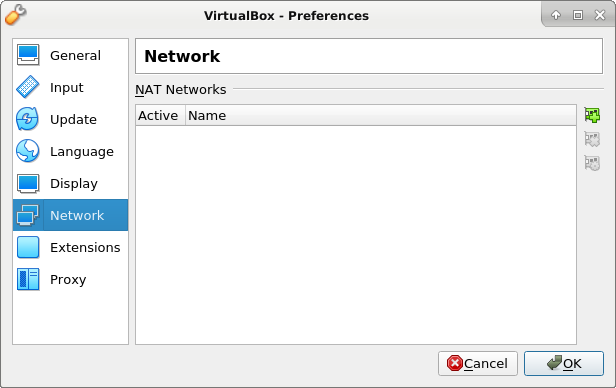
\includegraphics[width=0.99\linewidth]{linuxreader-img002.png}%
		}
		Click op het groene plusje aan de rechter kant.
		\end{minipage}

	\item
		\begin{minipage}[t]{\linewidth}
		\raggedright
		\adjustbox{valign=t}{%
			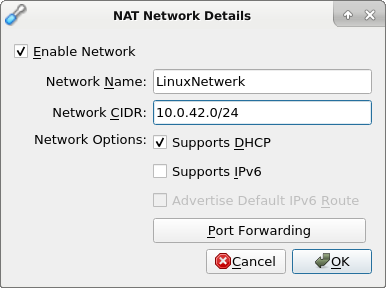
\includegraphics[width=0.99\linewidth]{linuxreader-img003.png}%
		}
		Geef het netwerk de naam ``LinuxNetwerk'' en een IP address range van 10.0.42.0. Click op OK om de wijzigingen op te slaan.
		\end{minipage}
\end{enumerate}


\section{Aanmaken van een Virtual Machine}
\begin{enumerate}
	\item 
		\begin{minipage}[t]{\linewidth}
		\raggedright
		\adjustbox{valign=t}{%
			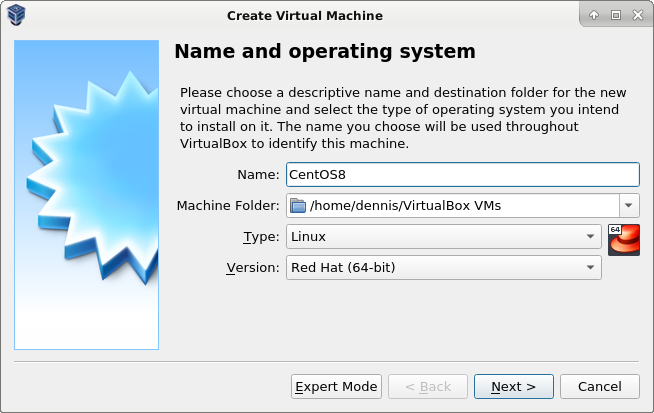
\includegraphics[width=0.99\linewidth]{linuxreader-img004.png}%
		}
		\end{minipage}
	\item Kies voor een 15 GB harddisk (VDI) die dynamisch mag groeien en 2 GB RAM.

	\item Als de machine aangemaakt is gaan we de netwerk settings wijzigen. We selecteren de machine en clicken op Properties. Bij Settings kiezen we voor Network.
	\item
		\begin{minipage}[t]{\linewidth}
		\raggedright
		\adjustbox{valign=t}{%
			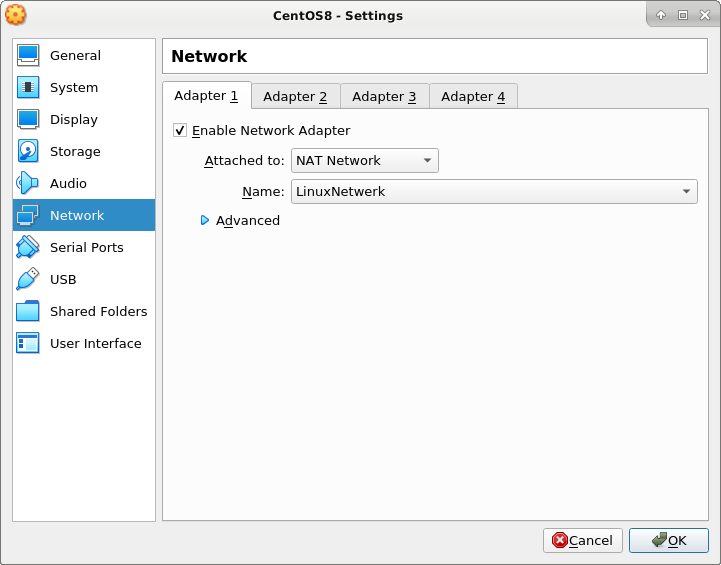
\includegraphics[width=0.99\linewidth]{linuxreader-img005.png}%
		}
		Wijzig bij Attached to: de setting naar NAT Network en selecteer vervolgens bij Name: het LinuxNewerk. Click op OK om de gemaakte wijzigingen op te slaan.
		\end{minipage}

\end{enumerate}

\section{CentOS installatie}
\begin{enumerate}
	\item
		\begin{minipage}[t]{\linewidth}
		\raggedright
		Verbindt de gedownloade ISO aan de virtuele CD speler door in het Settings menu op storage te clicken en het bestand te koppelen aan de CD.
		\adjustbox{valign=t}{%
			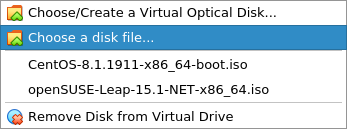
\includegraphics[width=0.99\linewidth]{linuxreader-img006.png}%
		}
		\end{minipage}
	\item Nu mag je de virtuele machine opstarten. Het eerste scherm dat je tegen komt geeft je de mogelijkheid om CentOS te installeren en dat gaan we dan ook doen.
	\item
		\begin{minipage}[t]{\linewidth}
		\raggedright
		Je kan wachten tot de installatie automatisch start of je drukt op enter om de installatie te starten.
		\adjustbox{valign=t}{%
			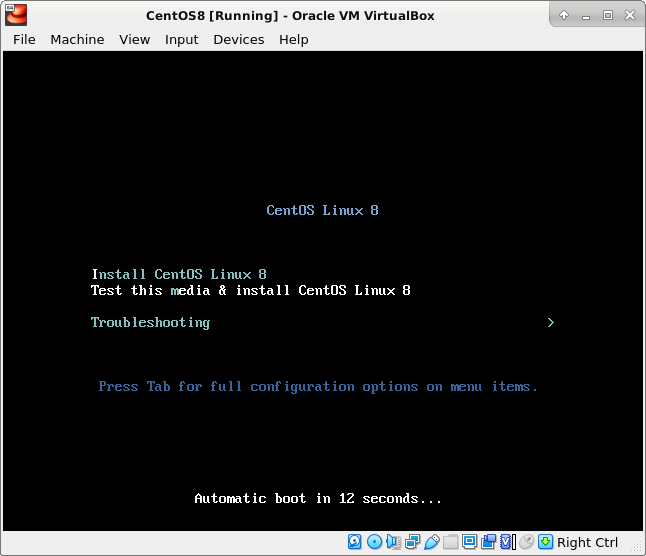
\includegraphics[width=0.99\linewidth]{linuxreader-img007.png}%
		}
		\end{minipage}
	\item
		\begin{minipage}[t]{\linewidth}
		\raggedright
		\adjustbox{valign=t}{%
			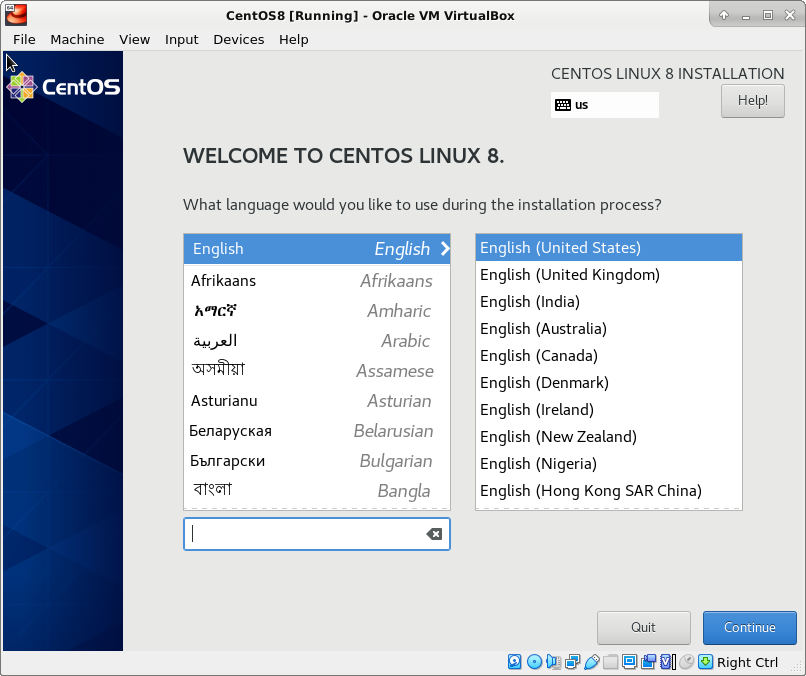
\includegraphics[width=0.99\linewidth]{linuxreader-img008.png}%
		}
		Het is misschien het handigst om een systeem in de Engelse taal te installeren, deze cursus gaat daarvan uit. Het grote voordeel is dat als je iets wil zoeken op het Internet dat je dan al gelijk in het Engels zoekt wat de kans op gelijksoortige problemen groter maakt er zijn immers meer mensen die Engels spreken dan Nederlands. Maar als je je niet vertrouwd genoeg vindt in het Engels dan kan je hier ook kiezen voor een Nederlandstalige installatie.
		\end{minipage}
	\item
		\begin{minipage}[t]{\linewidth}
		\raggedright
		In het vervolg scherm heb je heel veel keuzes in 1 keer. We zullen ze in de meest logische volgorde doorlopen.
		\adjustbox{valign=t}{%
			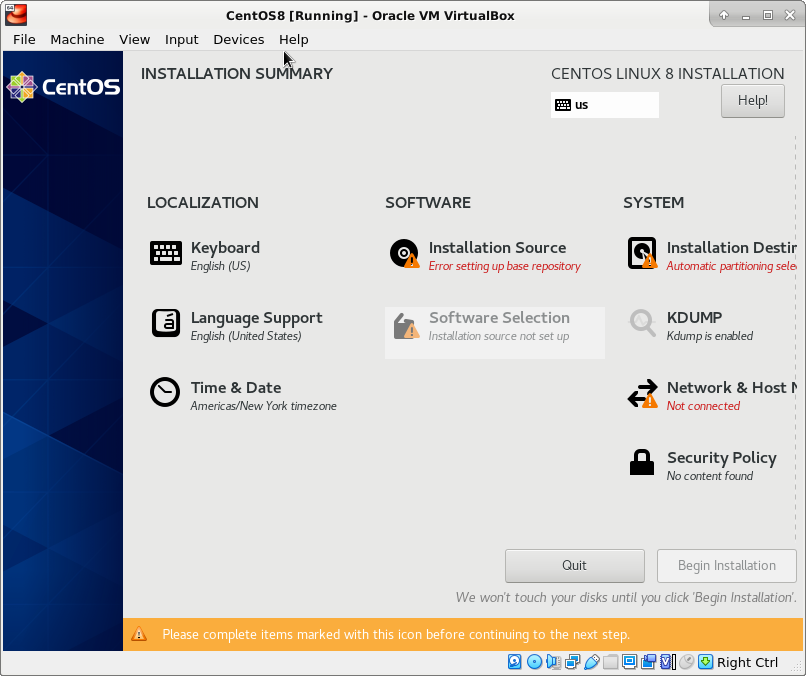
\includegraphics[width=0.99\linewidth]{linuxreader-img009.png}%
		}
		\end{minipage}
	\item We beginnen met Network \& Host Name. In het menu dat verschijnt hoef je het netwerk alleen maar op On te zetten en dan op Done te clicken.
	\item Vervolgens selecteren we Time \& Date en zetten we de tijdzone naar Europe en de plaats Amsterdam. En als dat nog niet aan staat dan zetten we Network time ook op On. Daarna clicken we weer Done.
	\item Nu gaan we voor de Installation Destination optie. Om het makkelijk te houden gaan we volledig voor de standaard instellingen, dus selecteren we Done.
	\item En als laatste kiezen we voor Installation Source. Aan de linkerkant selecteren we Workstation en aan de rechterkant zetten we een vinkje voor Office Suite and Productivity, we sluiten weer af met Done.
	\item Nu is de knop Begin Installation donker grijs geworden en kunnen we hem aanclicken.
	\item
		\begin{minipage}[t]{\linewidth}
		\raggedright
		Het systeem zal bezig gaan met de installatie en het geeft ons ondertussen de tijd om een wachtwoord voor root (Administrator van een Linux systeem) in te stellen en een gebruikersaccount voor onszelf te maken. Doe dit alle twee en zorg dat je de wachtwoorden goed onthoud of ergens opslaat.
		\adjustbox{valign=t}{%
			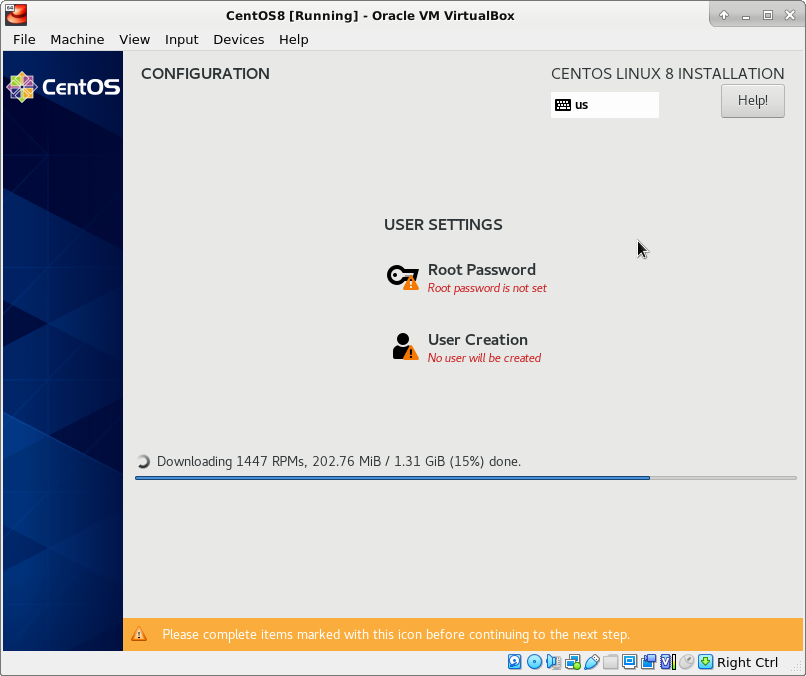
\includegraphics[width=0.99\linewidth]{linuxreader-img010.png}%
		}
		\end{minipage}
	\item Als de installatie klaar is dan moeten we via Settings $\rightarrow $ Storage de CD uit de virtuele CD speler verwijderen. Daarna kunnen we op Reboot clicken en zal ons nieuwe systeem opstarten.
	\item
		\begin{minipage}[t]{\linewidth}
		\raggedright
		\adjustbox{valign=t}{%
			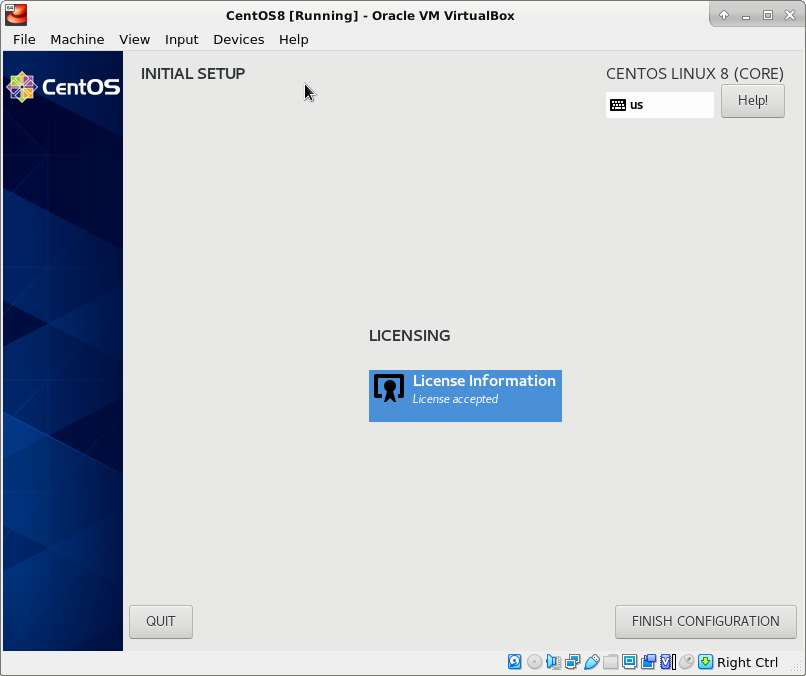
\includegraphics[width=0.99\linewidth]{linuxreader-img011.png}%
		}
		Na het opstarten en inloggen zal het systeem ons vragen om de licentievoorwaarden te accepteren.
		\end{minipage}

	\item Zodra je dit gedaan hebt kan je op FINISH CONFIGURATION clicken en zal de installatie worden afgerond.
	\item
		\begin{minipage}[t]{\linewidth}
		\raggedright
		\adjustbox{valign=t}{%
			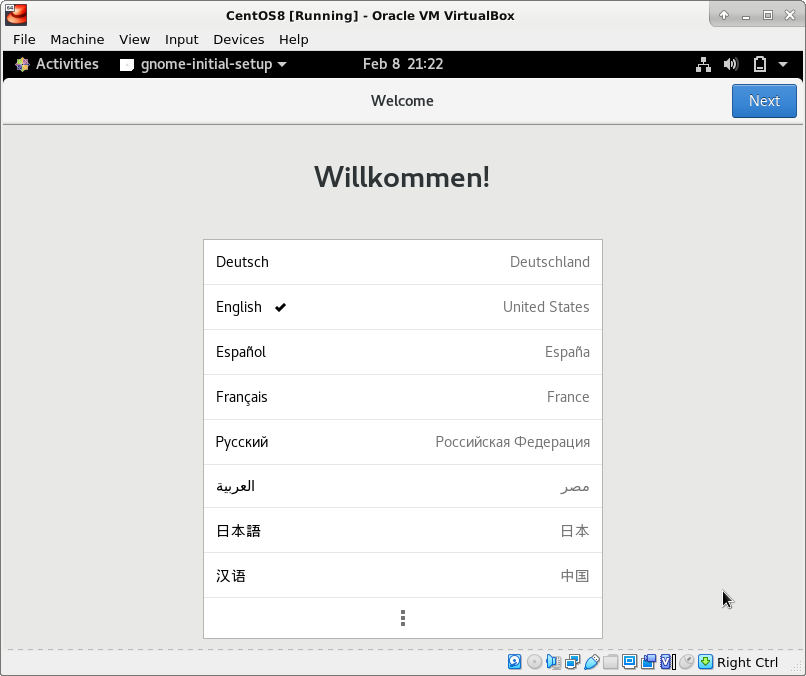
\includegraphics[width=0.99\linewidth]{linuxreader-img012.png}%
		}
		Je komt nu in het welkomstscherm terecht.
		\end{minipage}
	\item [META] Reinstall en zie wat er na Next komt en documenteer dit.
\end{enumerate}


\chapter{Werken met de grafische interface}
De Unix-wereld houdt erg van het paradigma ``Small is beautiful''. Daarmee bedoelen ze dat ze
graag kleine tools maken die \'e\'en ding goed doen. Dat zien we ook terug bij de grafische interface. Allereerst is er
een display server, dit is een stuk software dat ervoor zorgt dat er een grafische interface is. Het luistert naar de
muis en bestuurt de cursor en toont een grafisch scherm \ en dat is het wel zo'n beetje. Op deze grafische server
draait een window-manager. De window-manager vangt een applicatie in een frame (een window) en zorgt ervoor dat er naar
wens scrol-knoppen zijn en knopjes om het scherm te minimaliseren en/of te sluiten. Ook het achtergrondscherm is een
taak van de window-manager. Als laatste is er de desktop omgeving die zorgt voor de taakbalk, het configuratiescherm en
alle andere zaken die nodig zijn om van een desktop te kunnen spreken.

{\selectlanguage{dutch}
Als we dit allemaal hebben hebben we een desktop omgeving waarbinnen applicaties kunnen draaien.}

{\selectlanguage{dutch}
Er zijn twee dominante desktop omgevingen beschikbaar op de verschillende Linux distributies en dat zijn KDE en GNOME.
Naast deze twee zijn er nog vele verschillende anderen, maar die zullen we hier niet bespreken.}

{\selectlanguage{dutch}
\foreignlanguage{dutch}{KDE was de eerste van de twee genoemde desktopomgevingen en is gebaseerd op de Qt-library. In
het begin was de Qt-library geen open source vandaar dat er een concurrerent project is ontstaan. Later is het met Qt
helemaal goed gekomen en nu behoort ze tot de open source gemeenschap.}}

{\selectlanguage{dutch}
GNOME was het concurrerende project dat gestart werd omdat Qt niet open source was. Voor GNOME tot stand kwam was er een
open source fotomanipulatiepakket dat The \index{GIMP}GIMP heet, zie later in dit hoofdstuk. Om het pakket te kunnen
maken hadden de ontwikkelaars een grafische library ontwikkeld die GTK werd genoemd. Veel van wat er nodig is voor een
desktop zat daar al in en dus gebruikte het GNOME project de GTK-library als basis.}

{\selectlanguage{dutch}
\foreignlanguage{dutch}{De grafische interface kan enorm verschillen per distributie. Het maakt al enorm veel verschil
of je KDE of GNOME gebruikt als desktop omgeving. Laat je hierdoor niet imponeren, het wijst zich vaak vanzelf. KDE
ligt qua interface het dichtst tegen Windows aan, en zal dus het makkelijkst zijn om naar over te stappen. CentOS
gebruikt GNOME en vergt iets meer doorzettingsvermogen om te doorgronden.}}

{\selectlanguage{dutch}
\foreignlanguage{dutch}{Mocht het scherm in zijn screensaver vallen dan kan je door te clicken een scherm krijgen waarop
de tijd te zien is en met de {\textless}Enter{\textgreater} toets kom je op een login scherm en kan je in loggen met je
gebruikers wachtwoord.}}

{\selectlanguage{dutch}
\foreignlanguage{dutch}{Door op Activities te clicken krijg je extra scherm elementen te zien. Het nog een keer
aanclicken van Activities verbergt de elementen weer waardoor je meer ruimte op je scherm hebt voor applicaties.}}



\begin{figure}[H]
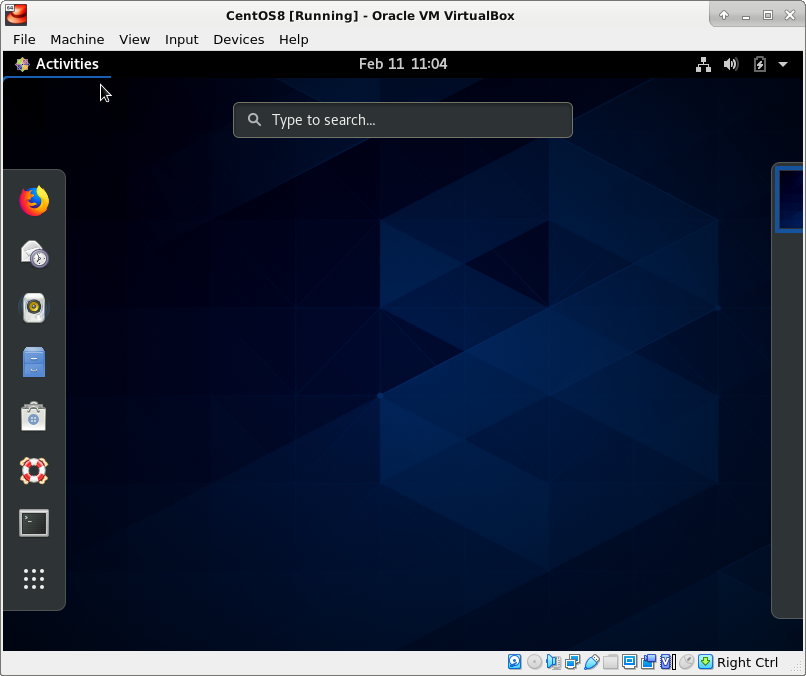
\includegraphics[width=0.9\textwidth]{linuxreader-img013.png}
\end{figure}
\begin{figure}[H]
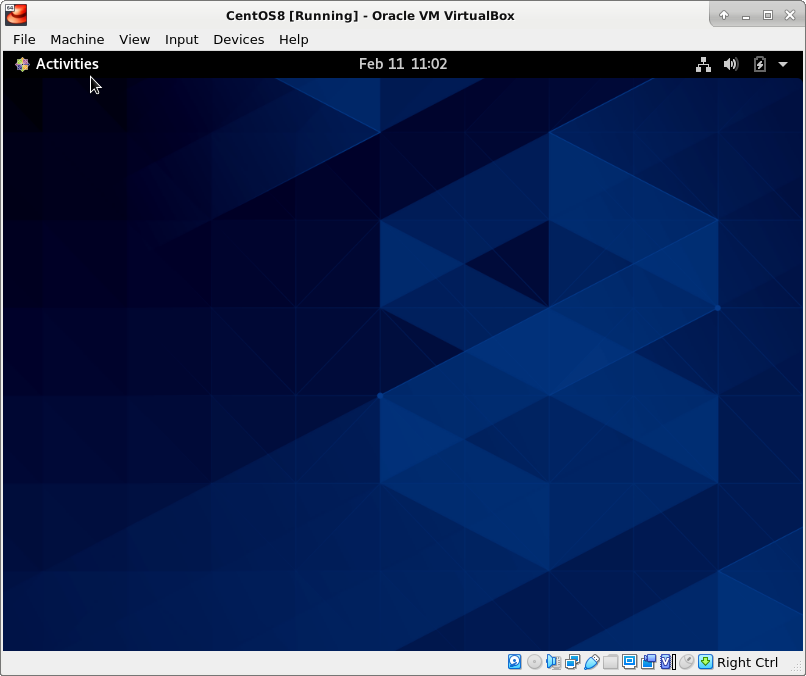
\includegraphics[width=0.9\textwidth]{linuxreader-img014.png}
\end{figure}

\section{Zoeken van bestanden of applicatie}
Met alle elementen op het scherm kan je de searchbar gebruiken om te zoeken op applicaties en bestanden. Als je zoekt op
Word, een Microsoft applicatie die niet op Linux beschikbaar is, dan vind je LibreOffice Writer een gratis en open
source alternatief. Start de applicatie op.

{\selectlanguage{dutch}
Neem de tekst over van het plaatje hierboven en zorg dat dit een eerste hoofdstuk titel wordt door de stijl te
veranderen. We gaan het document later vullen. Selecteer File en Save as{\dots} om het bestand op te slaan als
Document1.}

\begin{figure}[H]
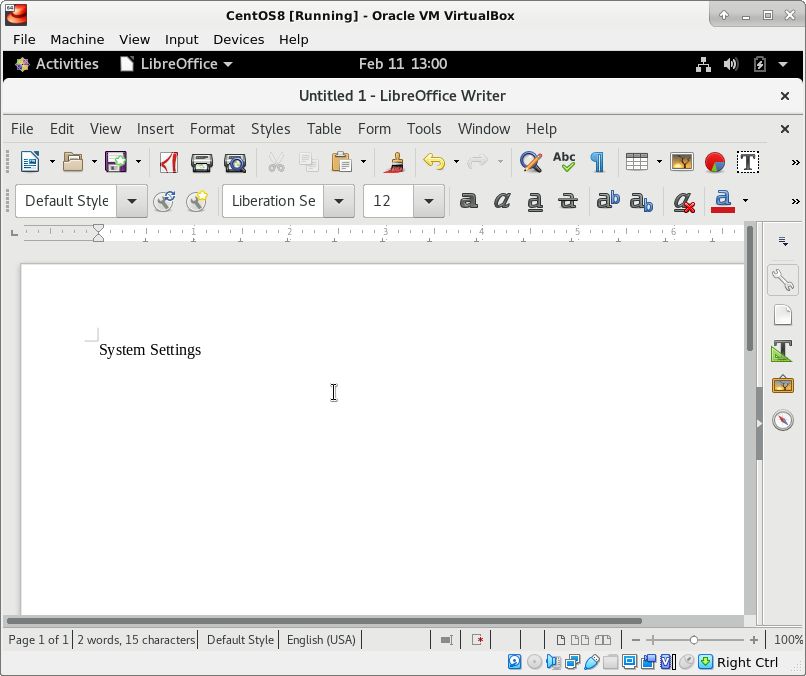
\includegraphics[width=0.9\textwidth]{linuxreader-img015.png}
\end{figure}
{\selectlanguage{dutch}
\foreignlanguage{dutch}{Meer over LibreOffice en de verschillende onderdelen van dit office pakket komt later aan de
orde als we Office Pakketten gaan bespreken. Nu concentreren we ons eerst op de beschikbare scherm elementen.}}

\section{Systeem configuratie}
Op de donkere balk waarop ook Activities staat vind je aan de rechterkant een naar beneden wijzend driehoekje. Het
aanklikken van het driehoekje geeft een menu met daarop een overzicht van de helderheid van het scherm, aan welk
netwerk je gekoppeld bent, als je een laptop gebruikt wat de batterij status is, je loginnaam en drie knopjes die je
van links naar rechts toegang geven tot de systeemsettings, het locken van je scherm en het uitzetten of herstarten van
je machine.



\begin{figure}[H]
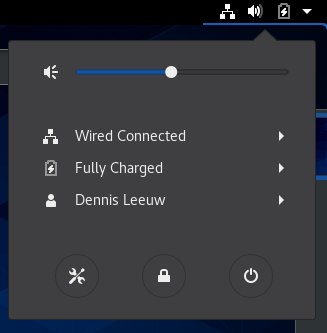
\includegraphics[width=0.9\textwidth]{linuxreader-img016.png}
\end{figure}
{\selectlanguage{dutch}
Selecteer Settings, scroll naar beneden naar Devices en selecteer deze, click dan op Displays. Trek het scherm los van
de topbar en schuif hem naar links. Click op de 800x600 resolutie en zet deze naar 1024x768}

{\selectlanguage{dutch}
\foreignlanguage{dutch}{Click op de Apply knop rechtsboven aan het scherm en daarna op Keep Settings. Natuurlijk mag je
resolutie ook hoger zetten, maar de minimale resolutie waarmee GNOME op CentOS 8 op een virtual machine prettig werkt
zonder dat je steeds met windows moet slepen is 1024x768. Selecteer {\textless} in de balk van Devices om terug te
komen in het hoofdmenu voor Settings. Loop door de verschillende opties om te ervaren waar je welke configuratie items
kan vinden en wijzigen.}}

\begin{figure}[H]
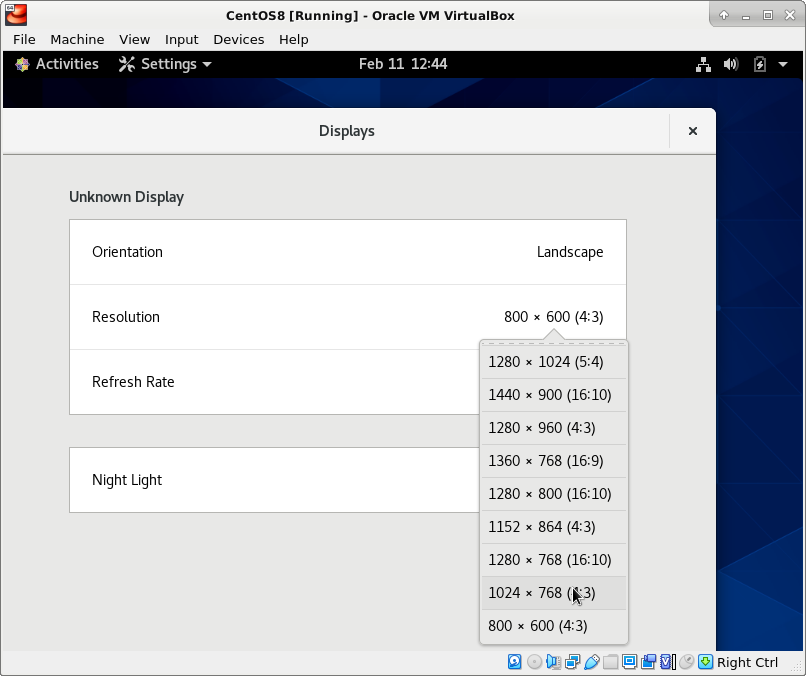
\includegraphics[width=0.9\textwidth]{linuxreader-img017.png}
\end{figure}
{\selectlanguage{dutch}
\foreignlanguage{dutch}{[TODO] Opdracht met documentatie in Writer om iets op te zoeken en te documenteren in Document1.
}}


\section{The Dash}
Aan de linkerkant van je scherm heb je de Dash, ook bekend als de Dock, applicatie bar of taskbar. Als je met je muis over de iconen van de taskbar gaat dan zie je per icoon wat deze betekent. Van boven naar beneden kom je het volgende tegen.

\begin{figure}[H]

\includegraphics[width=0.7811in,height=4.7398in]{linuxreader-img018.png}
\end{figure}
\begin{itemize}
\item Firefox -- een webbrowser
\item Evolution -- Een e-mail client
\item Rhythmbox -- een muziekspeler
\item Files -- Bestandsbrowser
\item Software -- Softwarebeheer
\item Help -- Documentatie
\item Terminal -- Toegang tot de console
\item Show applications -- een beperkt overzicht van beschikbare applicaties.
\end{itemize}

In de volgende hoofdstukken zullen we deze elementen doorlopen maar in een bredere context. We zullen bijvoorbeeld niet alleen Firefox behandelen, maar webbrowsers in zijn algemeenheid.


\section{Webbrowsers}
Een populaire browser is Mozilla \index{Firefox}Firefox. Het KDE-project heeft zijn eigen webbrowser. De KDE browser bestaat uit een engine
en en een interface. De engine is een library die alle benodigde functies voor het afhandelen van webpagina's heeft.
Het is ooit begonnen als KHTML. \ , de engine van deze browser,
\index{WebKit}WebKit wordt inmiddels ook door Apple gebruikt voor
zijn Safari browser.

Toen Google zijn eigen webbrowser ontwikkelde werd de basis hiervan vrij gegeven als open source
browser met de naam \index{Chromium}Chromium. Google gebruikt zelf
ook deze basis voor zijn Chrome browser, maar voegt daar nog wat eigen elementen aan toe. De open source versie is ook
op Linux te gebruiken en wordt door veel distributies meegeleverd en is makkelijk later te installeren.

[TODO] Basisgebruik firefox


\section{E-mail clients}
Mozilla levert naast de browser Firefox ook een open source \index{e-mail!e-mail client}e-mail client met de naam
\index{Thunderbird}Thunderbird dit is een volwaardige e-mail client inclusief kalenderfunctionaliteit.

{\selectlanguage{dutch}
Een e-mail client die erg lijkt op Microsoft Outlook is \index{Evolution}Evolution. Sinds versie 2.8 is het onderdeel
van de GNOME project en Evolution is dan ook standaard ge\"installeerd op CentOS.}

{\selectlanguage{dutch}
Evolution en Thunderbird draaien ook op Windows en Mac OS X.}

{\selectlanguage{dutch}
Het KDE project heeft ook zijn eigen e-mail client en die heet \index{KMail}KMail. Standaard zijn er dus al vele e-mail
clients om uit te kiezen. Als je Op Internet gaat zoeken zijn er nog veel meer smaken beschikbaar. Dat is een van de
vele voordelen van open source, anderen zeggen een nadeel, er zijn enorm veel keuzes.}

{\selectlanguage{dutch}
[TODO] basis gebruik Evolution koppelen met google account (IMAP)}

\section{Office pakketten}
Jaren lang was het meest gebruikte en dominante office pakket dat van Microsoft. Het was
beschikbaar voor Windows en Mac OS, maar niet voor Linux systemen. Oorspronkelijk had een Duitse student, Marco
B\"orries, StarWriter ontwikkeld om zijn studie in te documenteren. Later richtte hij een bedrijf op genaamd Star
Division en werd het een office pakket met de naam StarOffice. Het bedrijf werd in 1999 opgekocht door Sun Microsystems
die het pakket open source maakte onder de naam OpenOffice.org.

{\selectlanguage{dutch}
\foreignlanguage{dutch}{In 2009 werd Sun Microsystems gekocht door Oracle. Er was veel twijfel over wat Oracle met
OpenOffice.org wilde en dat zorgde voor een fork, een kopie van de code, die bekend werd onder de naam LibreOffice in
2010 en beheerd wordt door The Document Foundation. Oracle bracht }\foreignlanguage{dutch}{uiteindelijk in 2011 de code
van OpenOffice.org onder bij de Apache Foundation, helaas zat toen het merendeel van de ontwikkelaars al bij
LibreOffice. Beide projecten bestaan nog steeds, maar de meeste distributies leveren LibreOffice mee.}}

{\selectlanguage{dutch}
\foreignlanguage{dutch}{LibreOffice gebruikt standaard het Open Document Format voor al zijn documenten en is gratis
beschikbaar. Voor Linux, Mac OS X en Windows kan je het pakket vanaf de website downloaden
}\href{https://www.libreoffice.org/}{https://www.libreoffice.org}\foreignlanguage{dutch}{, maar dat hoeven wij niet te
doen omdat we het al meege\"installeerd hebben tijdens de installatie van CentOS.}}

{\selectlanguage{dutch}
LibreOffice bevat de volgende software onderdelen}

\begin{itemize}
\item {\selectlanguage{dutch}
Writer -- Tekstverwerking}
\item {\selectlanguage{dutch}
Calc -- Spreadsheets}
\item {\selectlanguage{dutch}
Impress -- Presentaties}
\item {\selectlanguage{dutch}
Draw -- Tekenpakket}
\item {\selectlanguage{dutch}
Math -- Een formule editor}
\item {\selectlanguage{dutch}
Base -- Database}
\end{itemize}
{\selectlanguage{dutch}
LibreOffice maakt standaard gebruik van het Open Document Format. Een officieel erkent en gestandaardiseerd
bestandsformaat dat er voor zorgt dat data altijd weer te lezen is omdat exact beschreven is hoe een document opgebouwd
moet zijn. De belangrijkste bestandsformaten zijn:}

\begin{itemize}
\item {\selectlanguage{dutch}
odt -- Open Document Text}
\item {\selectlanguage{dutch}
ods -- Open Document Spreadsheet}
\item {\selectlanguage{dutch}
odp -- Open Document Presentation}
\item {\selectlanguage{dutch}
odi -- Open Document Image, bitmap format}
\item {\selectlanguage{dutch}
odg -- Open Document Graphic, vector format}
\item {\selectlanguage{dutch}
odf -- Open Document Formula}
\item {\selectlanguage{dutch}
odb -- Open Document Database}
\end{itemize}

\section{Grafische applicaties}


\subsection{The GIMP}
\begin{figure}[H]
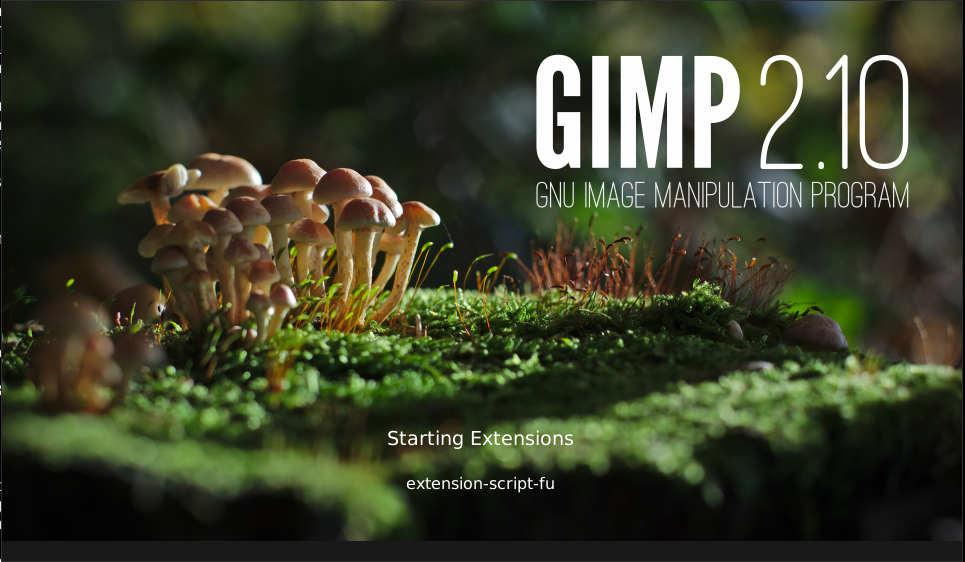
\includegraphics[width=\linewidth]{Gimp-splash.png}
\end{figure}

De GIMP is een applicatie om foto's te bewerken. Je kan het vergelijken met Photoshop van Adobe. Voor diegene die gewend zijn om te werken met Photoshop zal de interface aan de ene kant bekend voorkomen en aan de andere kant net even anders zijn.

\begin{figure}[H]
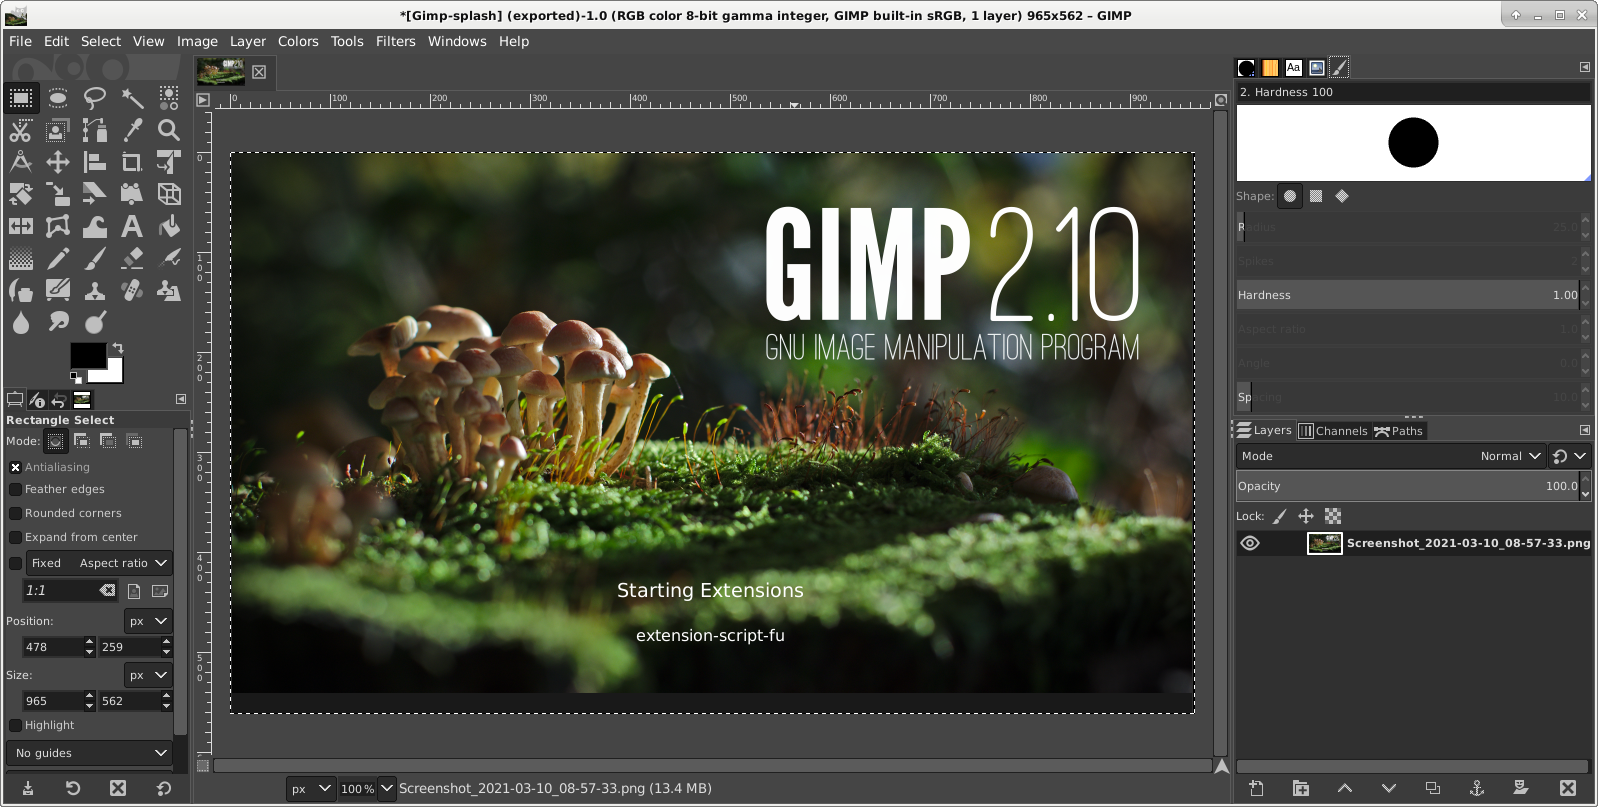
\includegraphics[width=\linewidth]{Gimp-work.png}
\end{figure}

\subsection{Inkscape}
\index{Inkscape}Inkscape is een applicatie om tekeningen in vectoren te maken. Het bouwt een tekening dus niet op in pixels zoals bijvoorbeeld BMP, jpeg of PNG, maar doet dit door punten met vectoren te beschrijven, hierdoor zijn tekeningen ``oneindig'' schaalbaar zonder kwaliteitsverlies.
\begin{figure}[H]
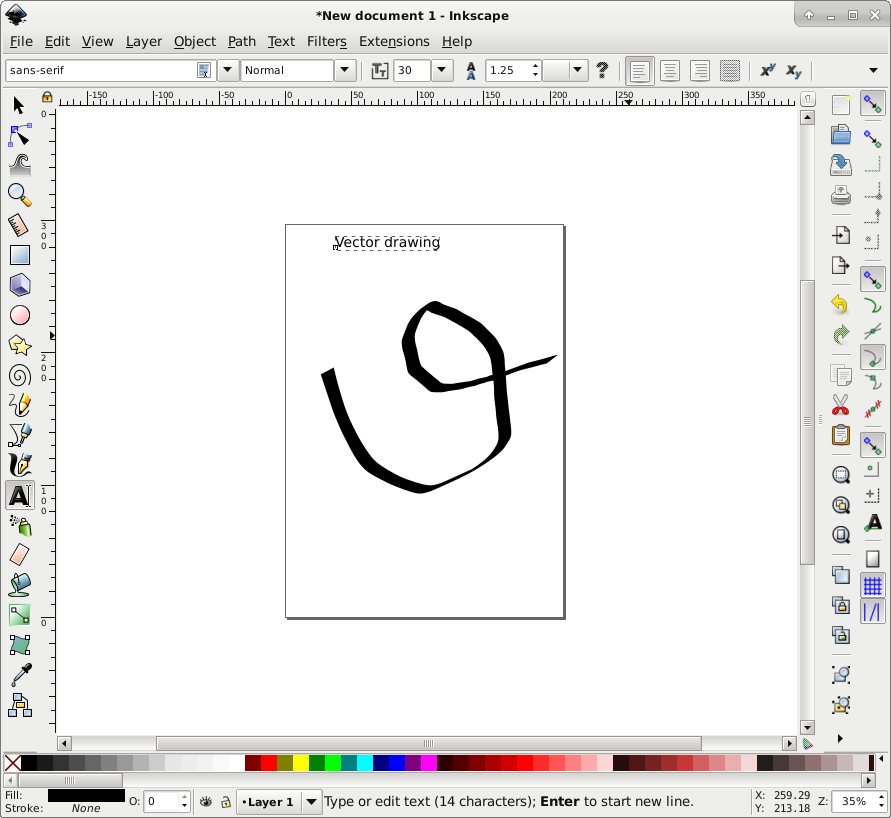
\includegraphics[width=\linewidth]{Inkscape-work.png}
\end{figure}



\section{Multimedia}
\subsection{Rhytmbox}
\subsection{VLC}
\subsection{KODI}
\section{Desktop publishing}
\subsection{Scribus}
Een open source document opmaak pakket is \index{Scribus}Scribus. Het is vergelijkbaar met Adobe Pagemaker.


\section{Bestandsbrowser}
\section{Installeren en updaten van software}
\subsection{Installeren van The GIMP}
\begin{figure}[H]
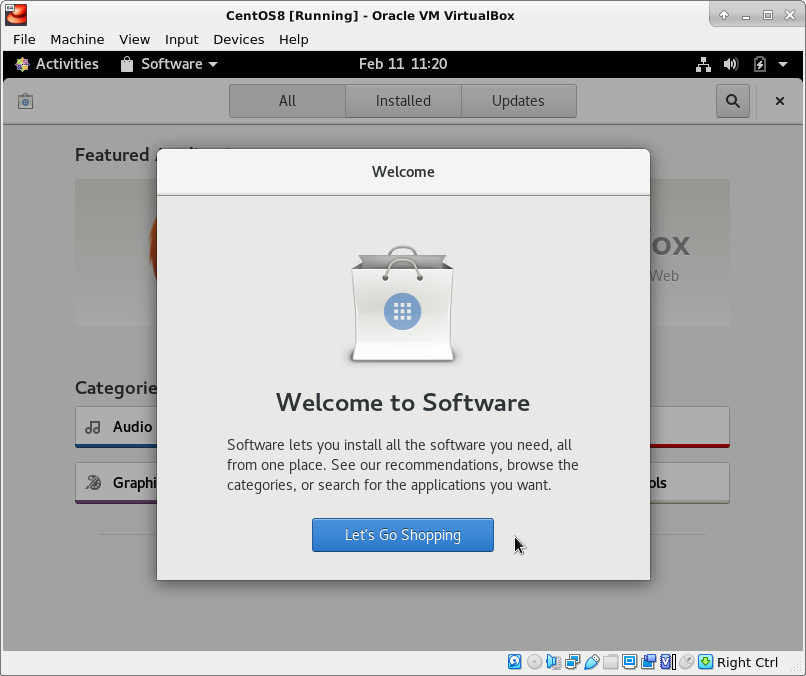
\includegraphics[width=0.9\textwidth]{linuxreader-img019.png}
\end{figure}
{\selectlanguage{dutch}
Rechtsboven kunnen we zoeken op een applicatie, we kunnen echter ook kiezen voor applicaties uit een Categorie. Klikken
we op Graphics \& Photography. Dan vinden we tussen de opties de Gimp. Selecteer de Gimp en klik Install. Er zal
gevraagd worden om het root-wachtwoord, na dit ingevoerd te hebben begint de installatie.}

{\selectlanguage{dutch}
Hierna kan je Software afsluiten of direct de Gimp opstarten.}

\begin{figure}
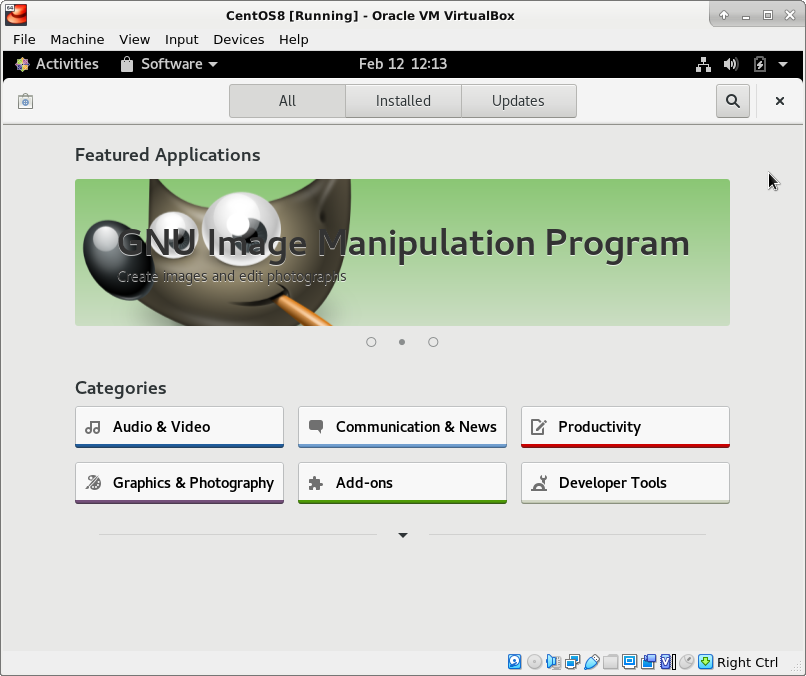
\includegraphics[width=0.9\textwidth]{linuxreader-img020.png}
\end{figure}

\section{Terminal}
De terminal applicatie wordt gebruikt om op de command line terecht te komen. Deze applicatie komt later uitgebreid aan
de orde. Hier slaan we hem over.

\section{Show applications}
Dit geeft een beperkt overzicht van de beschikbare applicaties. Voor snelle toegang tot de meest gebruikte applicaties
is dit een prima oplossing, verder is het makkelijker om gebruik te maken van de zoekfunctie zoals deze eerder in dit
document beschreven is.



%%%%%%%%%%%%%%%%%%%%%
%%% Index and End %%%
%%%%%%%%%%%%%%%%%%%%%
\backmatter
\printindex
\end{document}

%%% Last line %%%
